\chapter{Requirements Specification}
\label{ch:requirements}

This chapter is the single canonical requirements baseline for the thesis. It
states every requirement against the system as it is implemented at the current
source revision. Requirement identifiers (\texttt{FR-*}, \texttt{NFR-*}) are
stable and are the keys used by the traceability matrix in
Section~\ref{sec:traceability} and by the test-evidence families in the testing
chapter.

\section{System context, stakeholders, assumptions, and constraints}
\label{sec:context}

\subsection{System context}

The system is a research tool for discovering correct and efficient
\emph{dynamic} graph algorithms. A dynamic algorithm maintains a structural
result (a BFS tree, a DFS tree, a lexicographic BFS ordering, a strongly
connected component partition, or a reachability set) incrementally under edge
insertions and deletions, instead of recomputing it from scratch after every
change. The tool combines LLM-based code generation and repair with exhaustive,
isomorphism-aware verification inside an evolutionary search loop, and reports
both positive and negative results.

The system has one trusted side and many untrusted ones. The verifier, the
sandbox, and the evolutionary orchestrator are pre-built and trusted. Candidate
algorithms are untrusted Python written by an LLM; they execute only inside the
sandbox jail and are never given access to the verifier, the test graphs, the
oracle, or the host. That boundary is the central design constraint, stated as
a requirement in Section~\ref{sec:fr-ver} and \ref{sec:fr-sbx}.

The system is a Python package (\texttt{evoalgo}) with a command-line
interface, a local web user interface served from the same package, and a
harness mode in which an external coding agent drives the search while the
system only grades and records. There is no database; all state is JSON,
line-delimited JSON, and CSV under a per-run directory.

\subsection{Stakeholders}

\begin{itemize}
  \item \textbf{Researcher.} Configures and launches runs, monitors and steers
  them, inspects candidates, replays generation history, exports results, and
  runs the verifier self-test. The researcher is the primary actor and the one
  who interprets outcomes.
  \item \textbf{Supervisor.} Reviews run status, exported artefacts, and the
  verification evidence; audits the verifier and its acceptance evidence.
  \item \textbf{External coding agent.} In harness mode, a coding agent
  (for example enlcode, Claude Code, or Codex) edits the single candidate file
  and calls \texttt{evoalgo check}; the system grades and records each check.
  \item \textbf{LLM provider} (secondary actor). A hosted or local
  OpenAI-compatible model API, or an agent harness backend, that supplies the
  model calls for the generation, repair, and reflection roles.
\end{itemize}

\subsection{Assumptions}

\begin{itemize}
  \item A reachable model provider (hosted or local) is available for the
  duration of a run, or a scripted mock backend is used for offline tests.
  \item The host operating system is Linux with unprivileged user namespaces
  enabled, so the sandbox jail can be built. On a host without them the sandbox
  refuses to run unless explicitly disabled (see \texttt{FR-SBX-05}).
  \item The \texttt{nauty} graph data files are committed in the repository
  (\path{src/evoalgo/data/nauty/}); the \texttt{nauty} command line is not
  required at run time, only the pre-generated representative files.
  \item Dynamic outputs (BFS/DFS trees, orderings, partitions) are not unique;
  correctness is judged by an invariant or certificate, not by equality to a
  single reference output (Refinement R1, Section~\ref{sec:refinements}).
\end{itemize}

\subsection{Constraints}

\begin{itemize}
  \item \textbf{Platform.} Linux only, for the sandbox jail (namespaces and
  \texttt{mount\_setattr}). Python 3.11 or later.
  \item \textbf{No database.} Persistence is files only (JSON, JSONL, CSV).
  \item \textbf{No network for candidates.} Candidate code runs with the
  network namespace down; the verifier and agents use the network, the
  candidate never does.
  \item \textbf{Bounded verification.} Correctness is established by exhaustive
  finite testing within a stated graph-size and sequence bound, not by a
  proof (Refinement R3). The word ``proof'' is reserved for a mathematical or
  formal proof, which is out of scope.
\end{itemize}

\subsection{Non-goals}

\begin{itemize}
  \item A formal proof of correctness of a discovered algorithm beyond the
  stated bound. The Lean~4 formalisation step exists in the code but is
  experimental and never gates a run; it is not a committed deliverable.
  \item A general program synthesizer. The system targets a fixed set of
  dynamic graph problems with a fixed candidate interface; it does not
  synthesize arbitrary programs.
  \item A multi-user or remote service. The web UI binds to the loopback
  address and is intended for a single researcher on one host.
  \item Guaranteeing an efficiency improvement. The search may return a
  correct algorithm that is not faster than recomputing; that is a valid,
  reported outcome, not a failure.
\end{itemize}

\section{Use-case model}
\label{sec:usecases}

Figure~\ref{fig:use-cases} gives the use-case view.\footnote{The TikZ source of this figure was written with AI assistance (Claude Opus 5.5, Qwen3.8-27B) and checked against the code; see Section~\ref{sec:ai-use}.} Actors sit outside the
system boundary. White ellipses are triggered by a user or by the external
coding agent; grey ellipses are performed automatically by the system inside
the evolutionary loop or by the harness. \texttt{$\ll$include$\gg$} arrows run
from a base use case to the use case it always includes;
\texttt{$\ll$extend$\gg$} arrows run from an optional extension to the base it
conditions on.

\begin{figure}[H]
\centering
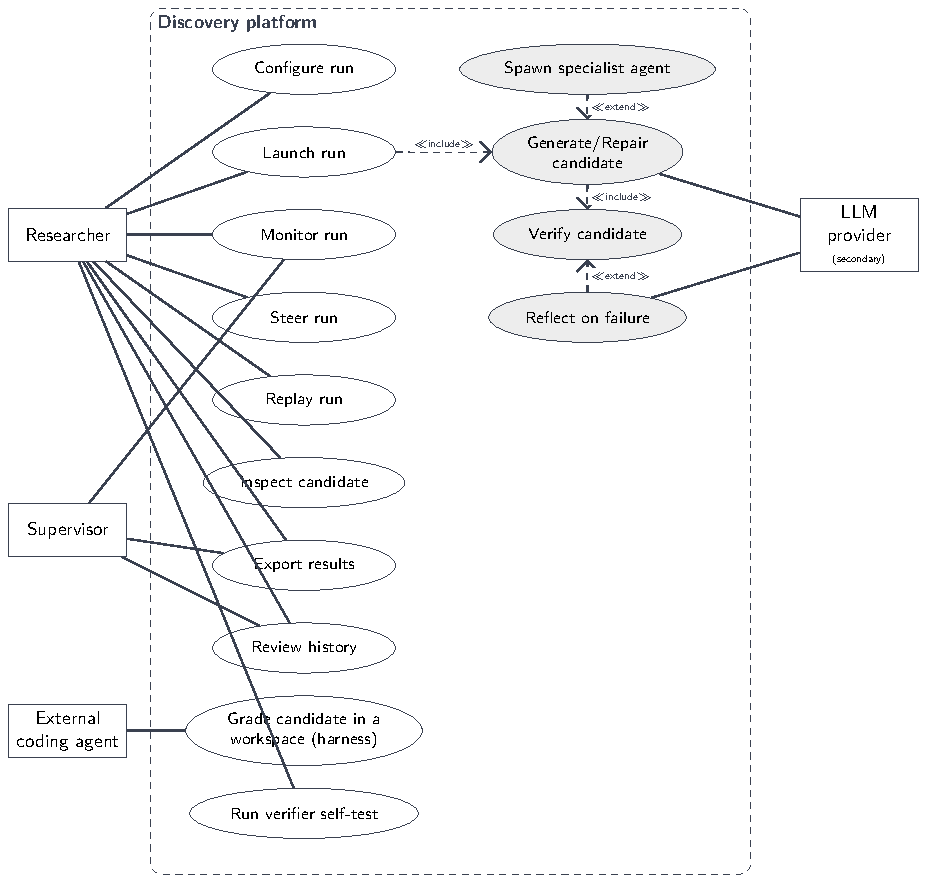
\includegraphics[width=0.85\textwidth]{figures/use-cases.pdf}
\caption{Use case diagram of the discovery platform. White ellipses are
user- or agent-triggered; grey ellipses are automatic. Reflection extends
verification (it runs only on a failure), and specialist spawning extends
generation (it runs only on a plateau).}
\label{fig:use-cases}
\end{figure}

The use cases are \emph{Configure run}, \emph{Launch run}, \emph{Monitor run},
\emph{Steer run}, \emph{Replay run}, \emph{Inspect candidate}, \emph{Export
results}, \emph{Review history}, \emph{Run verifier self-test}, and \emph{Grade
candidate in a workspace (harness)}, plus the internal \emph{Generate/Repair
candidate}, \emph{Verify candidate}, \emph{Reflect on failure}, and \emph{Spawn
specialist agent}. The five most important ones are summarised, each with its
actor, main flow and alternate and failure flows, in Table~\ref{tab:usecases}
(Appendix~\ref{app:tables}); their full narratives are in
Appendix~\ref{app:requirements}.


\section{Functional requirements}
\label{sec:fr}

The functional requirements are atomic and testable, and each has a stable
identifier whose prefix names the capability. There are 60: nine for the command
line and run control (\texttt{FR-CLI-01} to \texttt{09}), nine for the web
interface (\texttt{FR-UI}), eleven for the verification engine
(\texttt{FR-VER}), five for the sandbox (\texttt{FR-SBX}), seven for the agents
(\texttt{FR-AGENT}), ten for the evolutionary loop (\texttt{FR-EVO}), four for
persistence (\texttt{FR-PER}) and five for the harness (\texttt{FR-HAR}).
Table~\ref{tab:fr-summary} (Appendix~\ref{app:tables}) lists them by title and
priority; the full catalogue in Appendix~\ref{app:requirements} gives,
for every requirement, its input, precondition, behaviour, output, error or
rejection behaviour, priority, and acceptance evidence (named tests or campaign
artefacts). Priorities follow MoSCoW: \emph{Must} requirements are the
registered commitments, \emph{Should} and \emph{Could} requirements support them.



\section{Bounded verification universe}
\label{sec:universe}

The coverage claim of the verification engine is a finite, reproducible test
universe, not a proof. This section defines it so a reviewer can calculate its
size and distinguish exhaustive from sampled evidence.

\subsection{Base graphs}

Graphs are simple and loop-free, as an adjacency matrix of zeros and ones. The
base-graph set depends on the problem's direction and rooting:

\begin{itemize}
  \item \textbf{Directed, unrooted problems} use the non-isomorphic digraph
  representatives from the committed \texttt{nauty} data files
  (\texttt{directed\_n$<$n$>$.d6}), one per isomorphism class. The class counts
  for $n = 1$ to $5$ are 1, 3, 16, 218, and 9,608 (OEIS A000273, \citealp{oeisA000273}).
  \item \textbf{Directed, rooted problems} (BFS, DFS, reachability, which fix a
  source at vertex 0) use the rooted representatives
  (\texttt{rooted\_n$<$n$>$.d6}), one per (digraph, root-orbit) class with the
  root relabelled to vertex 0. The class counts for $n = 1$ to $5$ are 1, 4, 36,
  752, and 45,960 (OEIS A353996, \citealp{oeisA353996}).
  \item \textbf{Undirected problems} (MCS, LBFS) use \emph{every} labelled graph
  up to the bound, so the result does not depend on vertex labels. The labelled
  counts for $n = 2$ to $5$ are 2, 8, 64, and 1,024.
\end{itemize}

For directed problems the engine also applies a fixed number of deterministic
random relabellings of each representative (two per class for the final grade, one
for the search grade) to exercise label-dependent behaviour such as id
tie-breaks. A relabelling is isomorphic to its representative, so this adds
coverage of label handling without adding new isomorphism classes.

\subsection{Operation sequences}

For every base graph of size at most the exhaustive-flip bound (5), the universe
contains two kinds of sequences:

\begin{itemize}
  \item \textbf{All legal single-edge flips.} For each possible edge, one
  length-1 sequence that inserts it if absent or deletes it if present. This is
  ``every possible edge operation'' on the base graph: $n(n-1)$ flips for a
  directed graph and $n(n-1)/2$ for an undirected one.
  \item \textbf{Seeded random sequences.} \texttt{seq\_count} sequences of up to
  \texttt{seq\_len\_max} operations, each operation legal on the evolving graph,
  seeded by the bound seed plus the graph size, so the set is reproducible.
\end{itemize}

The defaults are \texttt{bound.n\_max} 5, \texttt{n\_random} 20,
\texttt{seq\_len\_max} 20, \texttt{seq\_count} 10, and \texttt{seed} 1337. The
\texttt{update\_mode} (\texttt{mixed}, \texttt{insert\_only},
\texttt{delete\_only}) filters the sequences to the allowed operation type while
keeping them legal.

\subsection{Exhaustive versus sampled}

Within the stated bound the universe is \emph{exhaustive up to isomorphism} for
directed problems (every non-isomorphic class, plus relabellings) and
\emph{exhaustive over labels} for undirected problems (every labelled graph).
Random sampling (\texttt{n\_random}) is used only for a graph size that has no
committed data file (that is, beyond the bound), so it never reduces coverage
inside the documented bound.

\subsection{Two grades and their exact sizes}

The engine uses two grades. The \emph{search grade} runs during the evolution on
every candidate: non-isomorphic graphs up to \texttt{search\_n\_max} (4), every
single flip, and \texttt{search\_seq\_count} (3) short sequences, with one
relabel per class; it takes seconds per candidate. The \emph{final grade} runs on
the best passing candidates on the full bound: $n \le 5$, every single flip, and
\texttt{seq\_count} (10) sequences of up to \texttt{seq\_len\_max} (20), with two
relabels per class.

The exact final-grade sizes, computed from the committed data files and the
sequence rules above, are:

\begin{center}
\footnotesize
\setlength{\tabcolsep}{6pt}
\begin{tabular}{@{}lrrrrr@{}}
\toprule
Problem & $n{=}2$ & $n{=}3$ & $n{=}4$ & $n{=}5$ & Total sequences \\
\midrule
Dynamic BFS / DFS (directed, rooted) & 96 & 1{,}728 & 49{,}632 & 4{,}136{,}400 & 4{,}187{,}856 \\
Dynamic LBFS (undirected, all labelled) & 22 & 104 & 1{,}024 & 20{,}480 & 21{,}630 \\
\bottomrule
\end{tabular}
\end{center}

These are the figures reported in the evaluation. A candidate that passes the
final grade has no counterexample within this bound; that is bounded exhaustive
verification, and it is not called a proof. The bound is on base graphs and on
the operation histories listed above: all single-edge flips and a finite set of
seeded sequences. It does not cover every internal state a candidate can reach
or arbitrarily long histories, even for $n \le 5$.

\section{Non-functional requirements}
\label{sec:nfr}

Each quality attribute has a measurable target or an explicit statement of what
is and is not asserted. The numbers are taken from the committed code, the test
suite, and the campaign artefacts; none is estimated.

\begin{itemize}
  \item \textbf{Performance.} A final grade of one BFS or DFS candidate on the
  full bound takes about 10 minutes (\texttt{NFR-PERF-01}), and a 1,000-graph
  chunk at $n = 5$ stays near 620 MB resident, inside the 4 GB address-space limit
  (\texttt{NFR-PERF-02}).
  \item \textbf{Security.} Candidate code is isolated from the host, the
  network and the secrets (\texttt{NFR-SEC-01}); secrets are handled by
  variable name only (\texttt{NFR-SEC-02}); the UI is loopback-only and
  token-protected (\texttt{NFR-SEC-03}).
  \item \textbf{Reliability.} A run resumes without losing completed work
  (\texttt{NFR-REL-01}), and transient model-call failures do not abort it
  (\texttt{NFR-REL-02}).
  \item \textbf{Reproducibility, usability, portability, maintainability.}
  The universe and parent selection are reproducible, model sampling is not
  (\texttt{NFR-REPR-01}); the UI is keyboard-usable without a WCAG claim
  (\texttt{NFR-USAB-01}); Linux and Python 3.11 or later
  (\texttt{NFR-PORT-01}); 193 pytest and 14 Vitest tests are the regression
  gate (\texttt{NFR-MAINT-01}).
\end{itemize}

Table~\ref{tab:nfr} in Appendix~\ref{app:tables} gives the measurement, the
threshold and the evidence for each of the eleven.

\section{Acceptance criteria per contribution}
\label{sec:acceptance}

Each registered contribution has a named demonstration or test, an explicit
pass/fail threshold, and a stored evidence artefact. Finite exhaustive testing
establishes bounded correctness within the stated bound; it is not a proof for
arbitrary graph size.

\begin{center}
\footnotesize
\setlength{\tabcolsep}{5pt}
\begin{longtable}{@{}>{\raggedright\arraybackslash}p{0.20\textwidth}>{\raggedright\arraybackslash}p{0.42\textwidth}>{\raggedright\arraybackslash}p{0.34\textwidth}@{}}
\toprule
\textbf{Contribution} & \textbf{Named demonstration / test} & \textbf{Threshold and evidence} \\
\midrule
\endfirsthead
\toprule
\textbf{Contribution} & \textbf{Named demonstration / test} & \textbf{Threshold and evidence} \\
\midrule
\endhead
\bottomrule
\endfoot

C1: research tool UI framework & A run is launched from the web New Run page,
monitored live, steered with a hint (acknowledged by the engine), and its
generation history is replayed with the scrubber, end to end. & The recorded
browser run completes with a final verdict and no error; the hint is acknowledged
at a generation boundary. Evidence: \texttt{ui\_check/01\_runs.png} through
\texttt{ui\_check/09\_failure\_drawer.png} and the recorded run
\texttt{runs/ui\_browser\_e2e\_bfs}. \\
\addlinespace[2pt]

C2: isomorphism-aware verification engine & The verifier self-test on the full
bound for a corpus problem: known-good references and equivalent controls
accepted, every seeded fault and one-line mutation rejected. & Zero false
negatives at $n \le 5$ (every seeded fault of the corpus rejected) and every reference and control
accepted. Evidence: \texttt{selftest\_dfs\_n5.log} (22 faults rejected, including
15 seeded and 7 one-line mutations of the known dynamic DFS reference) and
\texttt{selftest\_lbfs\_n5.log} (12 faults rejected); \texttt{test\_real\_faults\_rejected\_n5},
\texttt{test\_known\_good\_references\_pass\_n5}. \\
\addlinespace[2pt]

C3: cooperative agents with dynamic generation & An unattended orchestrator run
on dynamic BFS reaches a correct candidate, and the dynamic-agent variant spawns
and retires specialists on a plateau. & A search-grade pass is reached within the
configured generations with no human intervention; the final grade of the kept
candidate passes the full bound. Evidence: the campaign runs
(\texttt{eval1} orchestrator arm, 9/9 final-grade PASS) and
\texttt{test\_mock\_run\_spawns\_and\_retires\_a\_specialist},
\texttt{test\_plateau\_on\_fitness\_or\_work\_ratio}. \\
\bottomrule
\caption{Acceptance criteria per registered contribution.}
\label{tab:acceptance}
\end{longtable}
\end{center}

\section{Traceability to the approved proposal}
\label{sec:traceability}

Table~\ref{tab:traceability} traces each registered contribution and deliverable
to the requirement identifiers in this chapter, to the design sections that will
carry them (Chapter~\ref{ch:design}), to the implementation sections
(Chapter~\ref{ch:implementation}), and to the test-evidence families
(Chapter~\ref{ch:testing}). No registered contribution is removed; the four
refinements in Section~\ref{sec:refinements} narrow or re-prioritise the
registered wording and are stated explicitly.

\begin{center}
\footnotesize
\setlength{\tabcolsep}{4pt}
\begin{longtable}{@{}>{\raggedright\arraybackslash}p{0.17\textwidth}>{\raggedright\arraybackslash}p{0.20\textwidth}>{\raggedright\arraybackslash}p{0.25\textwidth}>{\raggedright\arraybackslash}p{0.16\textwidth}>{\raggedright\arraybackslash}p{0.14\textwidth}@{}}
\toprule
\textbf{Commitment} & \textbf{Req.\ IDs} & \textbf{Design} & \textbf{Implem.} & \textbf{Tests} \\
\midrule
\endfirsthead
\toprule
\textbf{Commitment} & \textbf{Req.\ IDs} & \textbf{Design} & \textbf{Implem.} & \textbf{Tests} \\
\midrule
\endhead
\bottomrule
\endfoot

C1: research tool UI framework & \texttt{FR-CLI-01} to \texttt{FR-CLI-09},
\texttt{FR-UI-01} to \texttt{FR-UI-09}, \texttt{FR-PER-01} to \texttt{FR-PER-04} &
\S\ref{sec:design-architecture}, \S\ref{sec:design-ui},
\S\ref{sec:design-concurrency}, \S\ref{sec:design-persistence} &
\S\ref{sec:impl-ui} & TC-UI, TC-SRV, TC-EVO \\
\addlinespace[2pt]

C2: isomorphism-aware verification engine & \texttt{FR-VER-01} to
\texttt{FR-VER-11}, \texttt{FR-SBX-01} to \texttt{FR-SBX-05} &
\S\ref{sec:design-verifier}, \S\ref{sec:design-sandbox},
\S\ref{sec:design-domain} & \S\ref{sec:impl-verifier},
\S\ref{sec:impl-sandbox} & TC-VER, TC-SBX, TC-PER \\
\addlinespace[2pt]

C3: cooperative agents with dynamic generation & \texttt{FR-AGENT-01} to
\texttt{FR-AGENT-06}, \texttt{FR-EVO-01} to \texttt{FR-EVO-10} &
\S\ref{sec:design-agents}, \S\ref{sec:design-architecture},
\S\ref{sec:design-concurrency} & \S\ref{sec:impl-agents} &
TC-AG, TC-EVO \\
\addlinespace[2pt]

Deliverable: tiered evaluation (calibration BFS/DFS to open LBFS) &
\texttt{FR-VER-10}, \texttt{FR-VER-11}, \texttt{NFR-PERF-01} &
\S\ref{sec:design-verifier}, \S\ref{sec:design-domain} &
\S\ref{sec:impl-verifier} & TC-VER; campaign \texttt{analysis.md} \\
\addlinespace[2pt]

Deliverable: harness mode (Refinement R4) & \texttt{FR-HAR-01} to
\texttt{FR-HAR-05}, \texttt{FR-VER-09} & \S\ref{sec:design-agents},
\S\ref{sec:design-sandbox} & \S\ref{sec:impl-agents}, \S\ref{sec:impl-sandbox}
& TC-HAR, TC-SBX \\
\bottomrule
\caption{End-to-end traceability from the registered commitments to
requirements, design, implementation, and test evidence.}
\label{tab:traceability}
\end{longtable}
\end{center}

\section{Refinements of the registered topic}
\label{sec:refinements}

Four refinements relative to the registered wording are stated here so they are
visible and judgeable rather than hidden. None removes a registered contribution.

\begin{description}
  \item[R1: comparison by invariant or certificate, not raw equality.] The
  registered wording compares a candidate's output against offline
  recomputation. Dynamic BFS and DFS outputs are not unique (ties in the
  traversal), so raw equality would reject correct candidates. The offline
  oracle still defines the semantics and is the efficiency baseline (the work
  ratio), but the checker accepts any valid structure: for BFS the parent tree
  and distances are certified, for DFS the parent and discover/finish times are
  certified by laminarity and the absence of a forward-cross edge, and for LBFS
  the ordering is certified by the four-point property. This is a sound
  refinement of the verifier contract, not a change of what is being measured.
  \item[R2: LBFS is undirected.] Lexicographic BFS is defined on undirected
  graphs, so dynamic LBFS runs on undirected graphs (every labelled graph up to
  the bound); BFS, DFS, SCC, and reachability run on directed graphs. The
  registered wording listed LBFS as directed; that is corrected here.
  \item[R3: two-tier grading and bounded verification.] Every candidate is
  graded during the run on the small search bound ($n \le 4$), and the best
  passing candidates are graded on the full final bound ($n \le 5$, 4,187,856
  test sequences for BFS/DFS). A result is reported as bounded exhaustive
  verification, that is no counterexample within the stated bound, and is never
  called a proof.
  \item[R4: the verifier is also exposed as a harness.] Besides the built-in
  orchestrator, the same verifier is exposed to an external coding agent through
  a harness (\texttt{evoalgo init} and \texttt{evoalgo check}, packaged as an
  agent skill). This is an extra mode, evaluated as a baseline against the
  orchestrator, not a replacement for it.
\end{description}
